\section{User Manual}

\subsection{User Overview}

We consider as User the administrator of the honeypot. Because of the dangerousness of the main source (a collection of malicious files), we believe the user is a highly skilled programmer who has complete understanding of what he is doing. We do not provide any automatic system for installing the analysis engine in a safe environment, and there are endless possibilities for the fool user to compromize not only the platform or its own machinery, but also the entire network he's connected to, giving to the attackers every informations they need for a counter-attack (and consequently the loss of the most precious property of a web honeypot, its undetectability).

The following manual will be divided in three main parts:
\begin{description}
\item[Website Overview]: the user is responsible for the creation of the fake web applications and for its deployment on the proxy. We will describe how to configure the proxy and the gateway in order to let the website be accessible from the internet;
\item[File Analysis]: the administrator of the honeypot can interface with a database, obtaining informations about files and using the proper tools for their deobfuscation;
\item[Web Interface]: for sake of semplicity in the management of the platform, we developed a web interface in order to let the administrator to have a quick overview over the honeypot system and to inspect single clusters and files.
\end{description}

\section{Website Overview}
\label{sec:websiteOverview}

The user is responsible for running the websites. We host the websites on separate virtual machines created using VMWare vSphere. In order to simplify the process of creation of a new virtual machine, we provide a template of such a server, based on a custom version of Debian 6 with an already installed updated version of the services needed by any webserver and an LXC basic environment (chroot included).

The service installed in the template are:
\begin{description}
\item[Python]: Python\cite{python} is a general purpose, high-level programming language. Because of its unique combination of code readability and ease of use it's widely used in the world as a scripting language. Attackers commonly uploads python scripts and run them in order to steal informations.
\item[Perl]: One of the first scripting language used by attackers in the world, Perl\cite{perl} can be considered a ``parent'' of Python, and it's still used in many cases, especially for the development of BotNets. Most of the script built in Perl, however, can be considered legacy code and it's usage is in constant decrease.
\item [cURL]: cURL\cite{curl} is one of the main command line tools used for downloading remote files on a machine. Requests can be highly customizable and there exist wrappers for most of the programming languages. These two characteristics make cURL a very attractive target for attackers using this tool in their script for downloading second-stage files.
\item [build-essentials]: This is one of the most commonly downloaded debian packages, providing all necessary headers for C/C++ programming languages. Without the installation of the packages compilation of C source files is not possible, and therefore any attempt for privilege escalation.
\item[PHP]: All the Content Management Systems we used are based on PHP. This programming language\cite{php}, recursive backronym for ``PHP: Hypertext Preprocessor'', is specifically aimed for web development and it is also the programming language most commonly used by attackers for the development of Web Shells.
\item[Apache]: Apache\cite{apache} is a widely used web server application. The reason we based our web servers on this application is its ability to extend its functionalities with several plugins, thanks to the wide number of developers maintaining the platform. We are keen in updating the application as soon as a new release is published, as this is the only point of entrance for attackers.
\item[Mysql]: as for PHP, every CMS we use relies on MySQL\cite{mysql} database for information storage. This is the most common relational database management system for manage MySQL databases, build database structures, back up data, inspect status, and work with data records.
\end{description}

We strongly suggest not to install other packages or software on the virtual machine in order to constrain the attacking surface, even if the possibility
for a malicious user to successful exploit a privilege escalation obtaining full control over the web server is remote (cfr. Section ~\ref{sec:vwmwareserver}).

The only action requested by the user after activating the web machine is to modify the IP address of the machine to the network 10.0.2.0/24. This action is mandatory in order for the web-server to be available from the internet. Every machine is by default connected to the private network 10.0.3.0/24, reachable only from the inside network. This allows the user to set up the desired CMS (and related services) without being on the Internet. Once the web server is configured, the user should take a snapshot of the machine through the specific feature available in vSphere, in order for the system to automatically restore the machine to the snapshot when it's requested.

After deploying the webserver, the gateway must be informed of the new route available. This action is performed by adding a specific IpTables rule in the form of
%use center and file because it looks nice!
\begin{center}
\file{iptables -A PREROUTING -i tun0 -p tcp -m tcp --dport 800X -j DNAT --to-destination 10.0.2.X:80}
\end{center}

This specific rules instruct the gateway to modify every TCP packet coming the tun0 interface (the exit from the VPN tunnel with the Proxy Server) with a specific destination port with a new destination IP (the one belonging to the new machine) and the HTTP standard port, 80.

Once the gateway is set, we can directly test the connection by connecting via SSH to any proxy and manually requesting the web page just created.

The last step requested for the system to be aware of the existence of the new web server and properly serving requests coming from the internet is the configuration of the proxies.
Because of the distributed nature of our proxies, we conveniently set up a script (called ``deploy.py'') on the gateway. This script takes two input parameters: an HTML page, which has to be modified in order to add an anchor link to the new webserver, and a file with a list of paths in the form \emph{``/app'' =\textgreater ``http://XXX:800X/app''}, where the new path and name of application should be added to. It will then update every proxy server with an updated version of the HTML page and and a new version of the proxy script.

At the end of the execution of the script, the new machine becomes part of the platform and is reachable from the attackers.

\section{File Analysis}

File Analysis is performed on a separate machine for isolation. We wanted the administrator of the honeypot to be able to explore files, perform queries to the database and to use Transformer, our deobfuscation tool, for getting better informations about a single file.

Once connected via SSH to the analysis machine, the user finds a folder called ``uploaded\_files'' which is actually a soft-link to the path ``/data/files''. This is the main path where malicious files are stored. Files are divided according to the machine where they have been uploaded. Inside each folder related to a single web machine the tree of files are divided according to the date they first have been requested following a path ``year/month/date''.
Inside each date there is the collection of files uploaded and a DIFF folder. Inside this folder all differential snapshots are located insided different files according to the time (in the format ``hourminutesecond'') the snapshot has been taken (cfr Section ~\ref{sec:SectionReqAnalysis}).
Furthermore, the var folder provide the tree of the original ``/var/www/'' of each machine as it appears in the initial snapshot.

\begin{figure}
\dirtree{%
.1 files.
.2 web1.
.2 web2.
.2 \{other machines\}.
.2 webN.
.3 2013.
.4 01.
.4 02.
.4 \{other months\}.
.4 12.
.5 01.
.5 02.
.5 \{other days\}.
.5 31.
.6 file1.
.6 file2.
.6 fileN.
.6 DIFF.
.7 000001.
.7 000031.
.7 HHMMSS.
.8 fileModified1.
.8 fileModified2.
.8 fileModifiedN.
.3 var.
.4 \{content of /var/www/ folder on webN machine\}.
}
\caption{Example of tree structure of /data/files folder}
\label{fig:dirtree1}
\end{figure}

The files are stored with the original name where characters that can't be encoded in format ASCII-7 are removed. If no characters are available (that's it, when all characters are not ASCII-7 compatible) or if a file with the same name is already present in the same folder, the file will be named with an arbitrary incremental number. It must be noticed that for sake of storage optimization files are unique, when the system receives a file that has already been stored in our database, the new one will be discarded.

\section{Database Architecture}

Every single connection received, files uploaded and request toward external servers is stored on a MySQL database located in a separate machine and periodically updated. We do not provide a specific API for communicating with the database. However, the user willing to perform queries can directly connect with it using the user ``analysis''.
The database is composed by several tables, we will explain the most important and most useful ones.

\subsection{FILES}
\begin{table}[H]
\begin{center}
\begin{tabular}{|c|c|c|c|c|c|}
\hline
 \textit{Field} & \textit{Type} & \textit{Null} & \textit{Key} &
 \textit{Default} & \textit{Extra} \\
\hline
id & int(11) & NO & PRI & None & auto\_increment \\
machine & char(4) & NO & MUL & None &  \\
relpath & varchar(255) & NO &  & None &  \\
base\_date & datetime & NO &  & None &  \\
last\_mod & datetime & YES &  & None &  \\
size & int(11) & NO &  & None &  \\
md5 & char(32) & NO & MUL & None &  \\
times\_seen & int(11) & NO &  & None &  \\
base & tinyint(1) & YES & MUL & None &  \\
ip\_src & varchar(15) & YES &  & None &  \\
\hline
\end{tabular}
\caption{FILES Table.\label{tab:FILESCategories}}
\end{center}
\end{table}

Table ~\ref{tab:FILESCategories} is the fundamental table present in the system. Here we store every file ever seen in the system both malicious and benign.
Every time a file is uploaded the md5 is computed and checked. The system performs a lookup on this table in order to see if the same file was already present in the system. We consider two files are equal if they have the same md5 and they have been uploaded to the same machine. In this case we update the last\_mod entry, otherwise we just insert a new line.

\subsection{HASHES}
\begin{table}[H]
\begin{center}
\begin{tabular}{|c|c|c|c|c|c|}
\hline
 \textit{Field} & \textit{Type} & \textit{Null} & \textit{Key} &
 \textit{Default} & \textit{Extra} \\
\hline
md5 & char(32) & NO & PRI & None &  \\
path & varchar(350) & YES & MUL & None &  \\
base\_date & datetime & YES &  & None &  \\
last\_date & datetime & YES & MUL & None &  \\
id\_category & int(11) & YES & MUL & None &  \\
base\_shell & tinyint(1) & YES &  & 0 &  \\
base & tinyint(4) & YES &  & 0 &  \\
id\_comment & int(11) & YES &  & None &  \\
\hline
\end{tabular}
\caption{HASHES Table.\label{tab:HASHESCategories}}
\end{center}
\end{table}

Table ~\ref{tab:HASHESCategories} collects files uploaded on the system. The primary key is the md5, and every time an uploaded file was already present in the table we update the entry with a new last\_date.

\subsection{CLUSTERS}
\begin{table}[H]
\begin{center}
\begin{tabular}{|c|c|c|c|c|c|}
\hline
 \textit{Field} & \textit{Type} & \textit{Null} & \textit{Key} &
 \textit{Default} & \textit{Extra} \\
\hline
md5 & char(32) & YES &  & None &  \\
cluster\_id & int(11) & YES & MUL & None &  \\
cluster\_category\_id & int(11) & YES & MUL & None &  \\
\hline
\end{tabular}
\caption{CLUSTERS Table.\label{tab:CLUSTERSCategories}}
\end{center}
\end{table}

\subsection{TEST\_HASHES}
\begin{table}[H]
\begin{center}
\begin{tabular}{|c|c|c|c|c|c|}
\hline
 \textit{Field} & \textit{Type} & \textit{Null} & \textit{Key} &
 \textit{Default} & \textit{Extra} \\
\hline
md5\_original & char(32) & NO & PRI & None &  \\
md5\_normalized & char(32) & NO &  & None &  \\
ssdeep & varchar(116) & YES &  & None &  \\
sdhash & varchar(32000) & YES &  & None &  \\
\hline
\end{tabular}
\caption{TEST\_HASHES Table.\label{tab:TEST_HASHESCategories}}
\end{center}
\end{table}

Table ~\ref{tab:TEST_HASHESCategories} is the linking point between files and clusters. We store the md5 of each file before normalization, and the two values coming from the deobfuscation and normalization (cfr. section ~\ref{sec:Clustering}.

\subsection{FILES\_PER\_IP}
\begin{table}[H]
\begin{center}
\begin{tabular}{|c|c|c|c|c|c|}
\hline
 \textit{Field} & \textit{Type} & \textit{Null} & \textit{Key} &
 \textit{Default} & \textit{Extra} \\
\hline
ip & varchar(15) & NO &  & None &  \\
md5 & char(32) & NO &  & None &  \\
id & int(11) & YES &  & None &  \\
sure & tinyint(1) & YES &  & None &  \\
\hline
\end{tabular}
\caption{FILES\_PER\_IP Table.\label{tab:FILES_PER_IPCategories}}
\end{center}
\end{table}

We wanted to track the number of files uploaded by each IP. This table keeps track of this phenomenon, tracking for each file (according to the md5) the IP address uploading it. By grouping files uploaded for each IP address we can get informations like the average number of files uploaded by each address.

\subsection{DOMAIN\_TOTAL}
\begin{table}[H]
\begin{center}
\begin{tabular}{|c|c|c|c|c|c|}
\hline
 \textit{Field} & \textit{Type} & \textit{Null} & \textit{Key} &
 \textit{Default} & \textit{Extra} \\
\hline
id & int(11) & NO & PRI & None & auto\_increment \\
domain & varchar(255) & YES &  & None &  \\
totCountRequests & int(11) & YES &  & None &  \\
totCountIP & int(11) & YES &  & None &  \\
\hline
\end{tabular}
\caption{DOMAIN\_TOTAL Table.\label{tab:DOMAIN_TOTALCategories}}
\end{center}
\end{table}

Table ~\ref{tab:DOMAIN_TOTALCategories} relates information from each domain of provenance of each connection to the number of requests performed and to the number of different IP addresses connecting using it.

\subsection{REFERER\_TOTAL}
\begin{table}[H]
\begin{center}
\begin{tabular}{|c|c|c|c|c|c|}
\hline
 \textit{Field} & \textit{Type} & \textit{Null} & \textit{Key} &
 \textit{Default} & \textit{Extra} \\
\hline
id & int(11) & NO & PRI & None & auto\_increment \\
url & varchar(2000) & YES &  & None &  \\
totCountRequests & int(11) & YES &  & None &  \\
totCountIP & int(11) & YES &  & None &  \\
\hline
\end{tabular}
\caption{REFERER\_TOTAL Table.\label{tab:REFERER_TOTALCategories}}
\end{center}
\end{table}

Similar to the one used for the domains, Table ~\ref{tab:REFERER_TOTALCategories} collect data from the referer used by attackers while uploading their files.

It must be noticed that the database is far more complex and the user will find more tables than the one shown above. This is just a collection of the most useful ones for performing basic operations.

Each table and each column belonging to it is described in the database, available after directly connecting to it.

\section{Visualization}

Our aim is to create a honeypot platform which can be easily deployed, updated and monitored by the administrator of the system. In order to accomplish the last action we created a web interface for monitoring the health of the system and obtain feedbacks from the analysis of data.

\subsection{Back-End Architecture}

We chose to use \emph{Node.Js} as platform for developing the web server. \emph{Node.Js} is advertised on its website \cite{node_home} as
\begin{quotation}
Node.js is a platform built on Chrome's JavaScript runtime for easily building fast, scalable network applications. Node.js uses an event-driven, non-blocking I/O model that makes it lightweight and efficient, perfect for data-intensive real-time applications that run across distributed devices.
\end{quotation}

Its particular event-driven, non-blocking model, in fact, allows us to perform database queries and file analysis operations without involving waiting time from the end-user point of view. Furthermore, its modular nature and easiness of deployment makes the replication process fast and reliable.

We wanted to create a platform which does rely on a minimum number of external addition (other to the web server) and which can perform several parallel queries to different databases for computing rankings and other operations. The system relies on \emph{Express} \cite{express_node} Framework, which is specifically aimed for minimality and flexibility, and uses only a few other modules, in the specific \emph{mysql} driver for Database communications and \emph{sanitizer}, a sanitizer library for strings.

Another requirement we imposed to our software is the possibility for it to work in a private network, disconnected from the Internet. For this reason, every library is provided directly by the web server and there is no need to rely to any external server for the web interface to work.

\subsection{Front-End Architecture}

The Front-End architecture deeply relies on Javascript. We wanted to allow a good interactivity for the operator, who should be able to go from a high-level view to the single file analysis in a couple of clicks.

The interface uses Bootstrap \cite{bootstrap} framework: this is one of the most used front-end frameworks for web development, as it is able to create nice and clean web pages by creating a powerful templating system. It also manage interactions with end-users through several add-ons, like modals and accordions.

Graphs displaying is performed using D3 library \cite{d3_home} (acronym for Data-Driven Document), a library for displaying graphs as collections of SVG elements. Thanks to its emphasis on web standards, this library will work on all modern browsers (starting from Internet Explorer 8), without any issue, and avoiding to rely on proprietary frameworks for graph displaying. Other than static graphs like pie charts, this library is able to use heuristic algorithms in order  to show force-directed graphs, which have been one of our minimal requirements for clustering graphs visualization on our web interface.

\subsection{Overview}

Our dashboard should be able to give the following informations to the administrator: an overview over the current situation inside the system (files received, requests etc), an interactive graph showing in a clear way the various clusters, files the system failed to clusterize, statistics about the system (requests, common referrers, attackers provenance..). In the following we will give three examples of the functionalities of the interface.

\begin{figure}[tbh]
\centerline{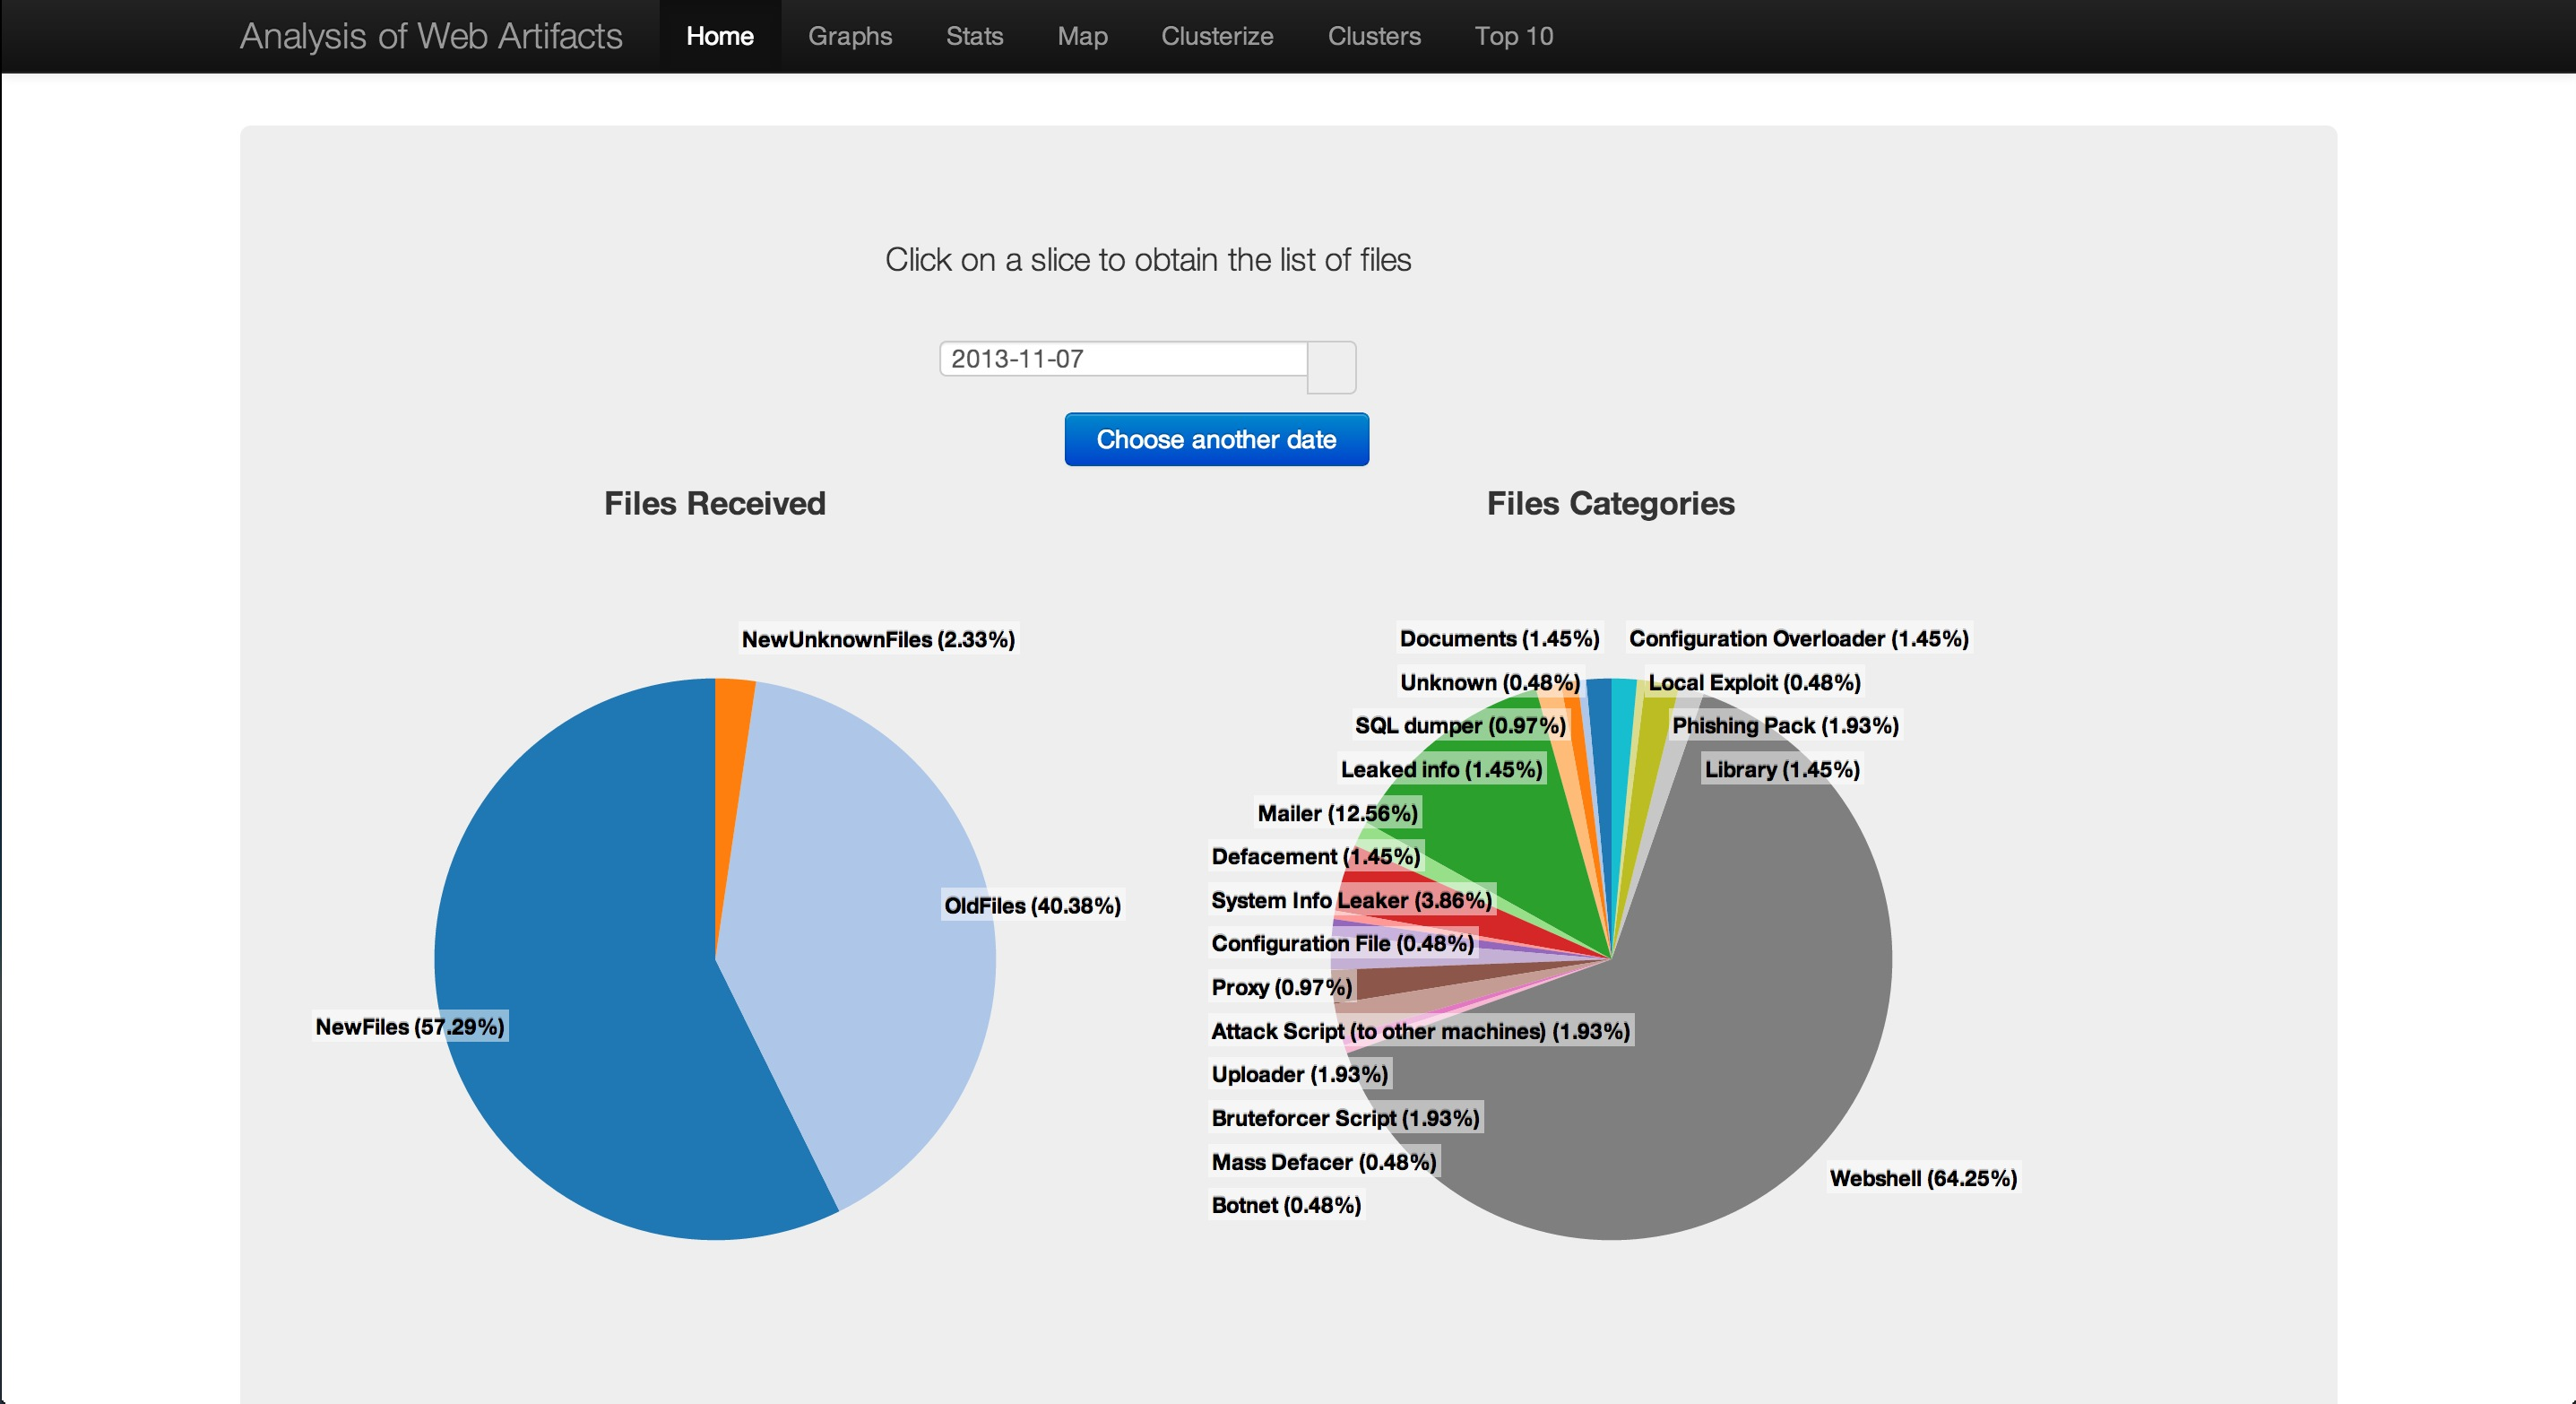
\includegraphics[scale=0.2]{Images/honeyFace_home.jpg}}
\caption{Screenshot of the web interface home page\label{fig:web_home}}
\end{figure}

The homepage(ref~\ref{fig:web_home}) of the web interface displays several pie charts, the most important being the number of file received during the day, divided among three categories, oldFiles (files that were already present in our databases), newFiles (new files received for which our clusterization system already categorized) and newUnknownFiles (new files that our system was unable to clusterize), and the result of our categorization for the files received during the day. Clicking on a slice of a pie displays a list of files belonging to that tranche, with the possibility to display details for each file.

\begin{figure}[tbh]
\centerline{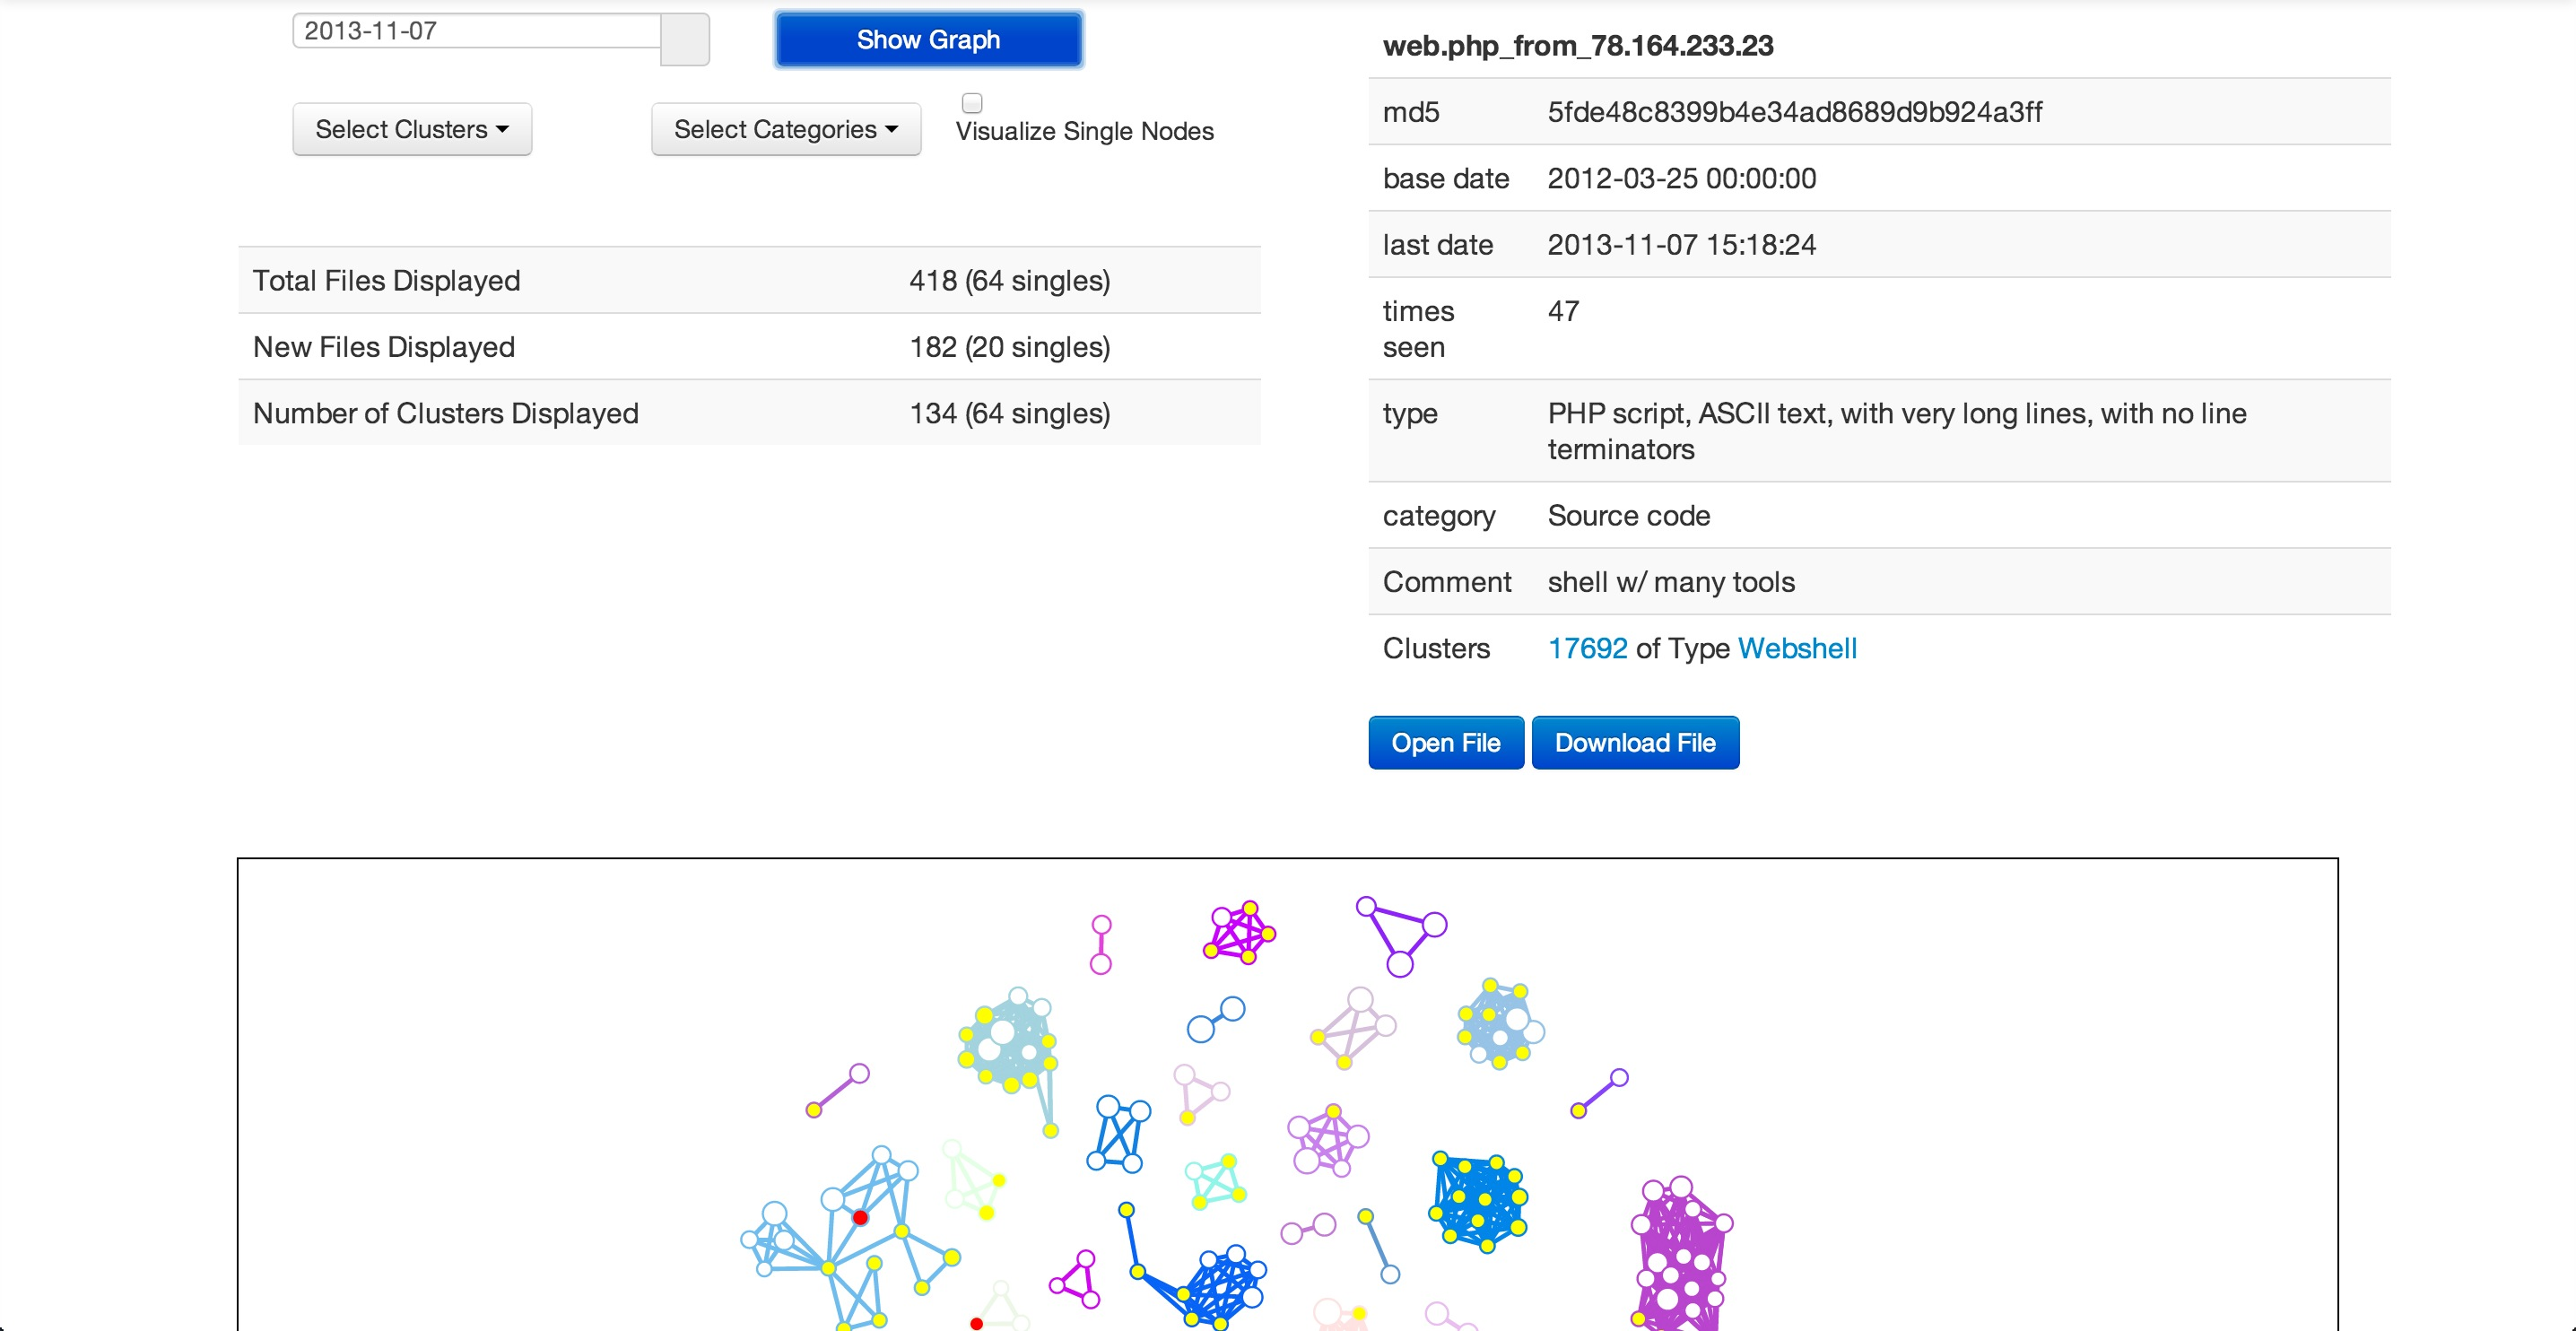
\includegraphics[scale=0.2]{Images/honeyFace_graph.jpg}}
\caption{Screenshot of a graph created by the web interface\label{fig:web_graph}}
\end{figure}

The Graph page (ref~\ref{fig:web_graph}) displays a force-directed graph showing the different clusters. It is possible to choose several parameters for the display, like the categories to be displayed and the file types. We chose to display files received only in the last 15 days with respect to the date chosen, in order not to overload the browser (the map is interactive and it's built client-side).

We can display details about a single file through the single file web page. We can see several details about the file, type, clusters, date received etc. We also have the possibility to write a comment about the file.
One of The most interesting features we provide on this page is the possibility to use ``Transformer'' over the single file (ref~\ref{fig:deobfDouble}), obtaining a rapid feedback over how our system managed the single file and in order to get a better understanding over the code.

\begin{figure}
\centering
\begin{subfigure}{.5\textwidth}
  \centering
  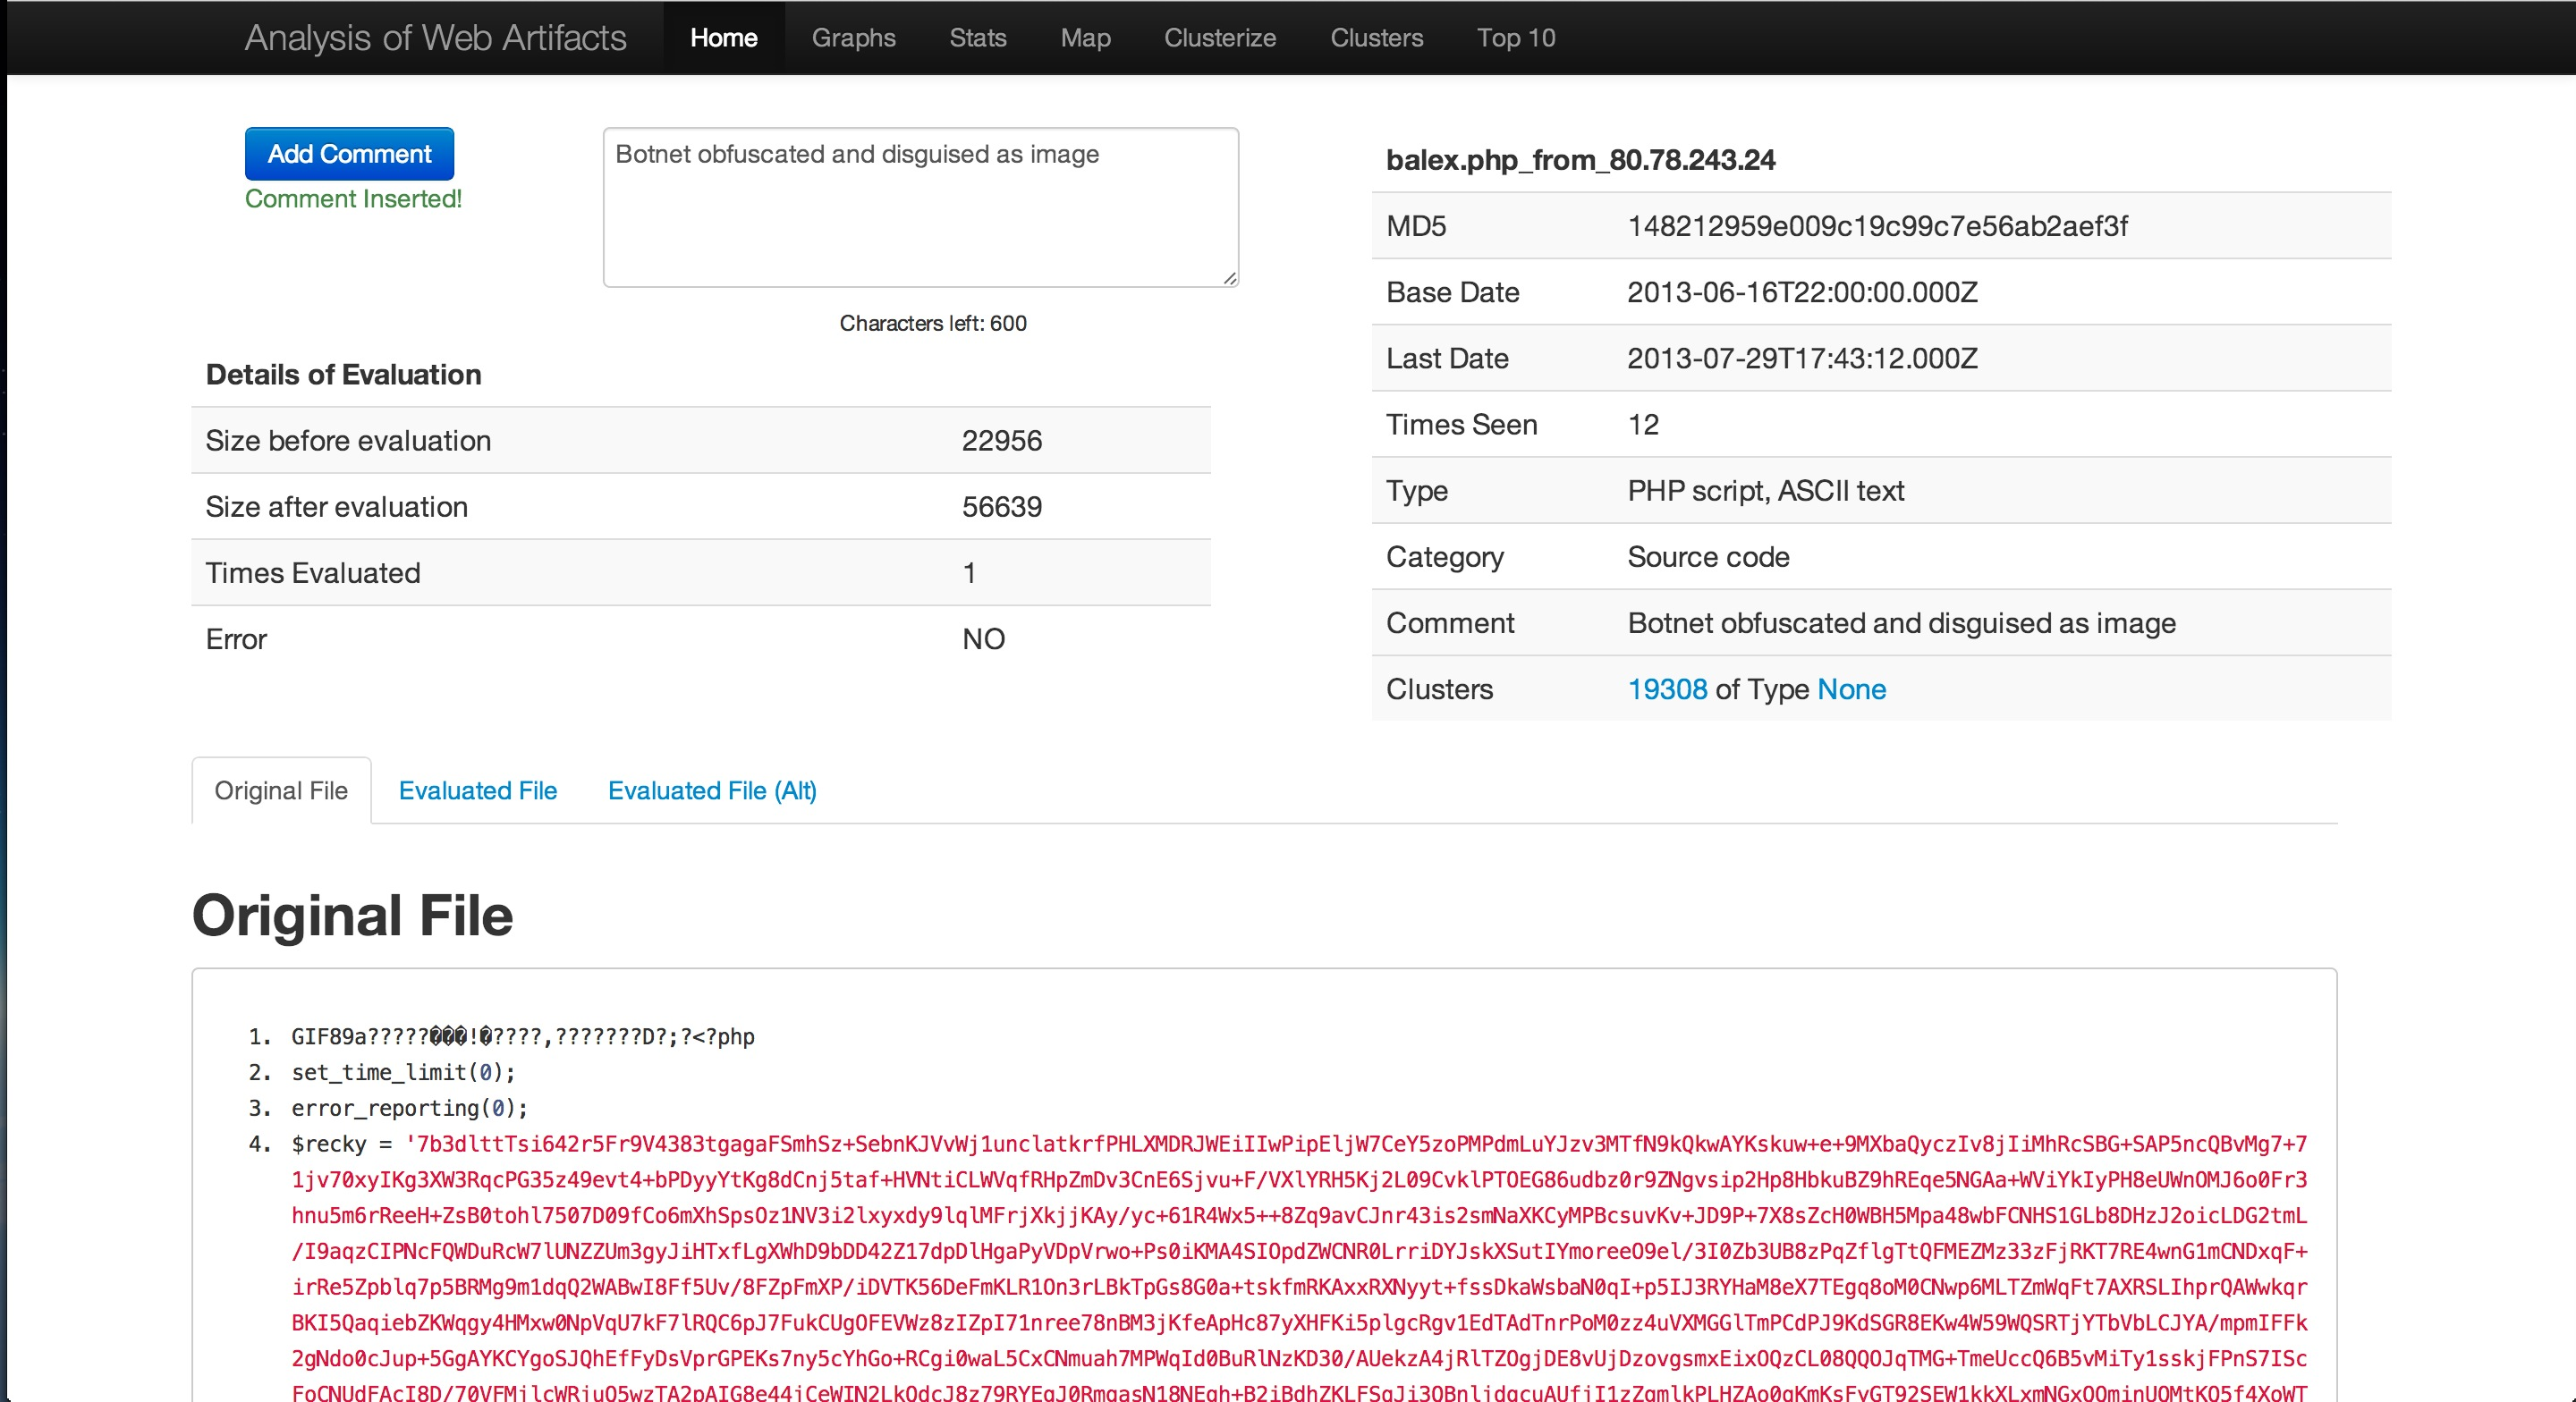
\includegraphics[width=1.0\linewidth]{Images/obf_file.jpg}
  \caption{Before deobfuscation}
  \label{fig:sub1}
\end{subfigure}%
\begin{subfigure}{.5\textwidth}
  \centering
  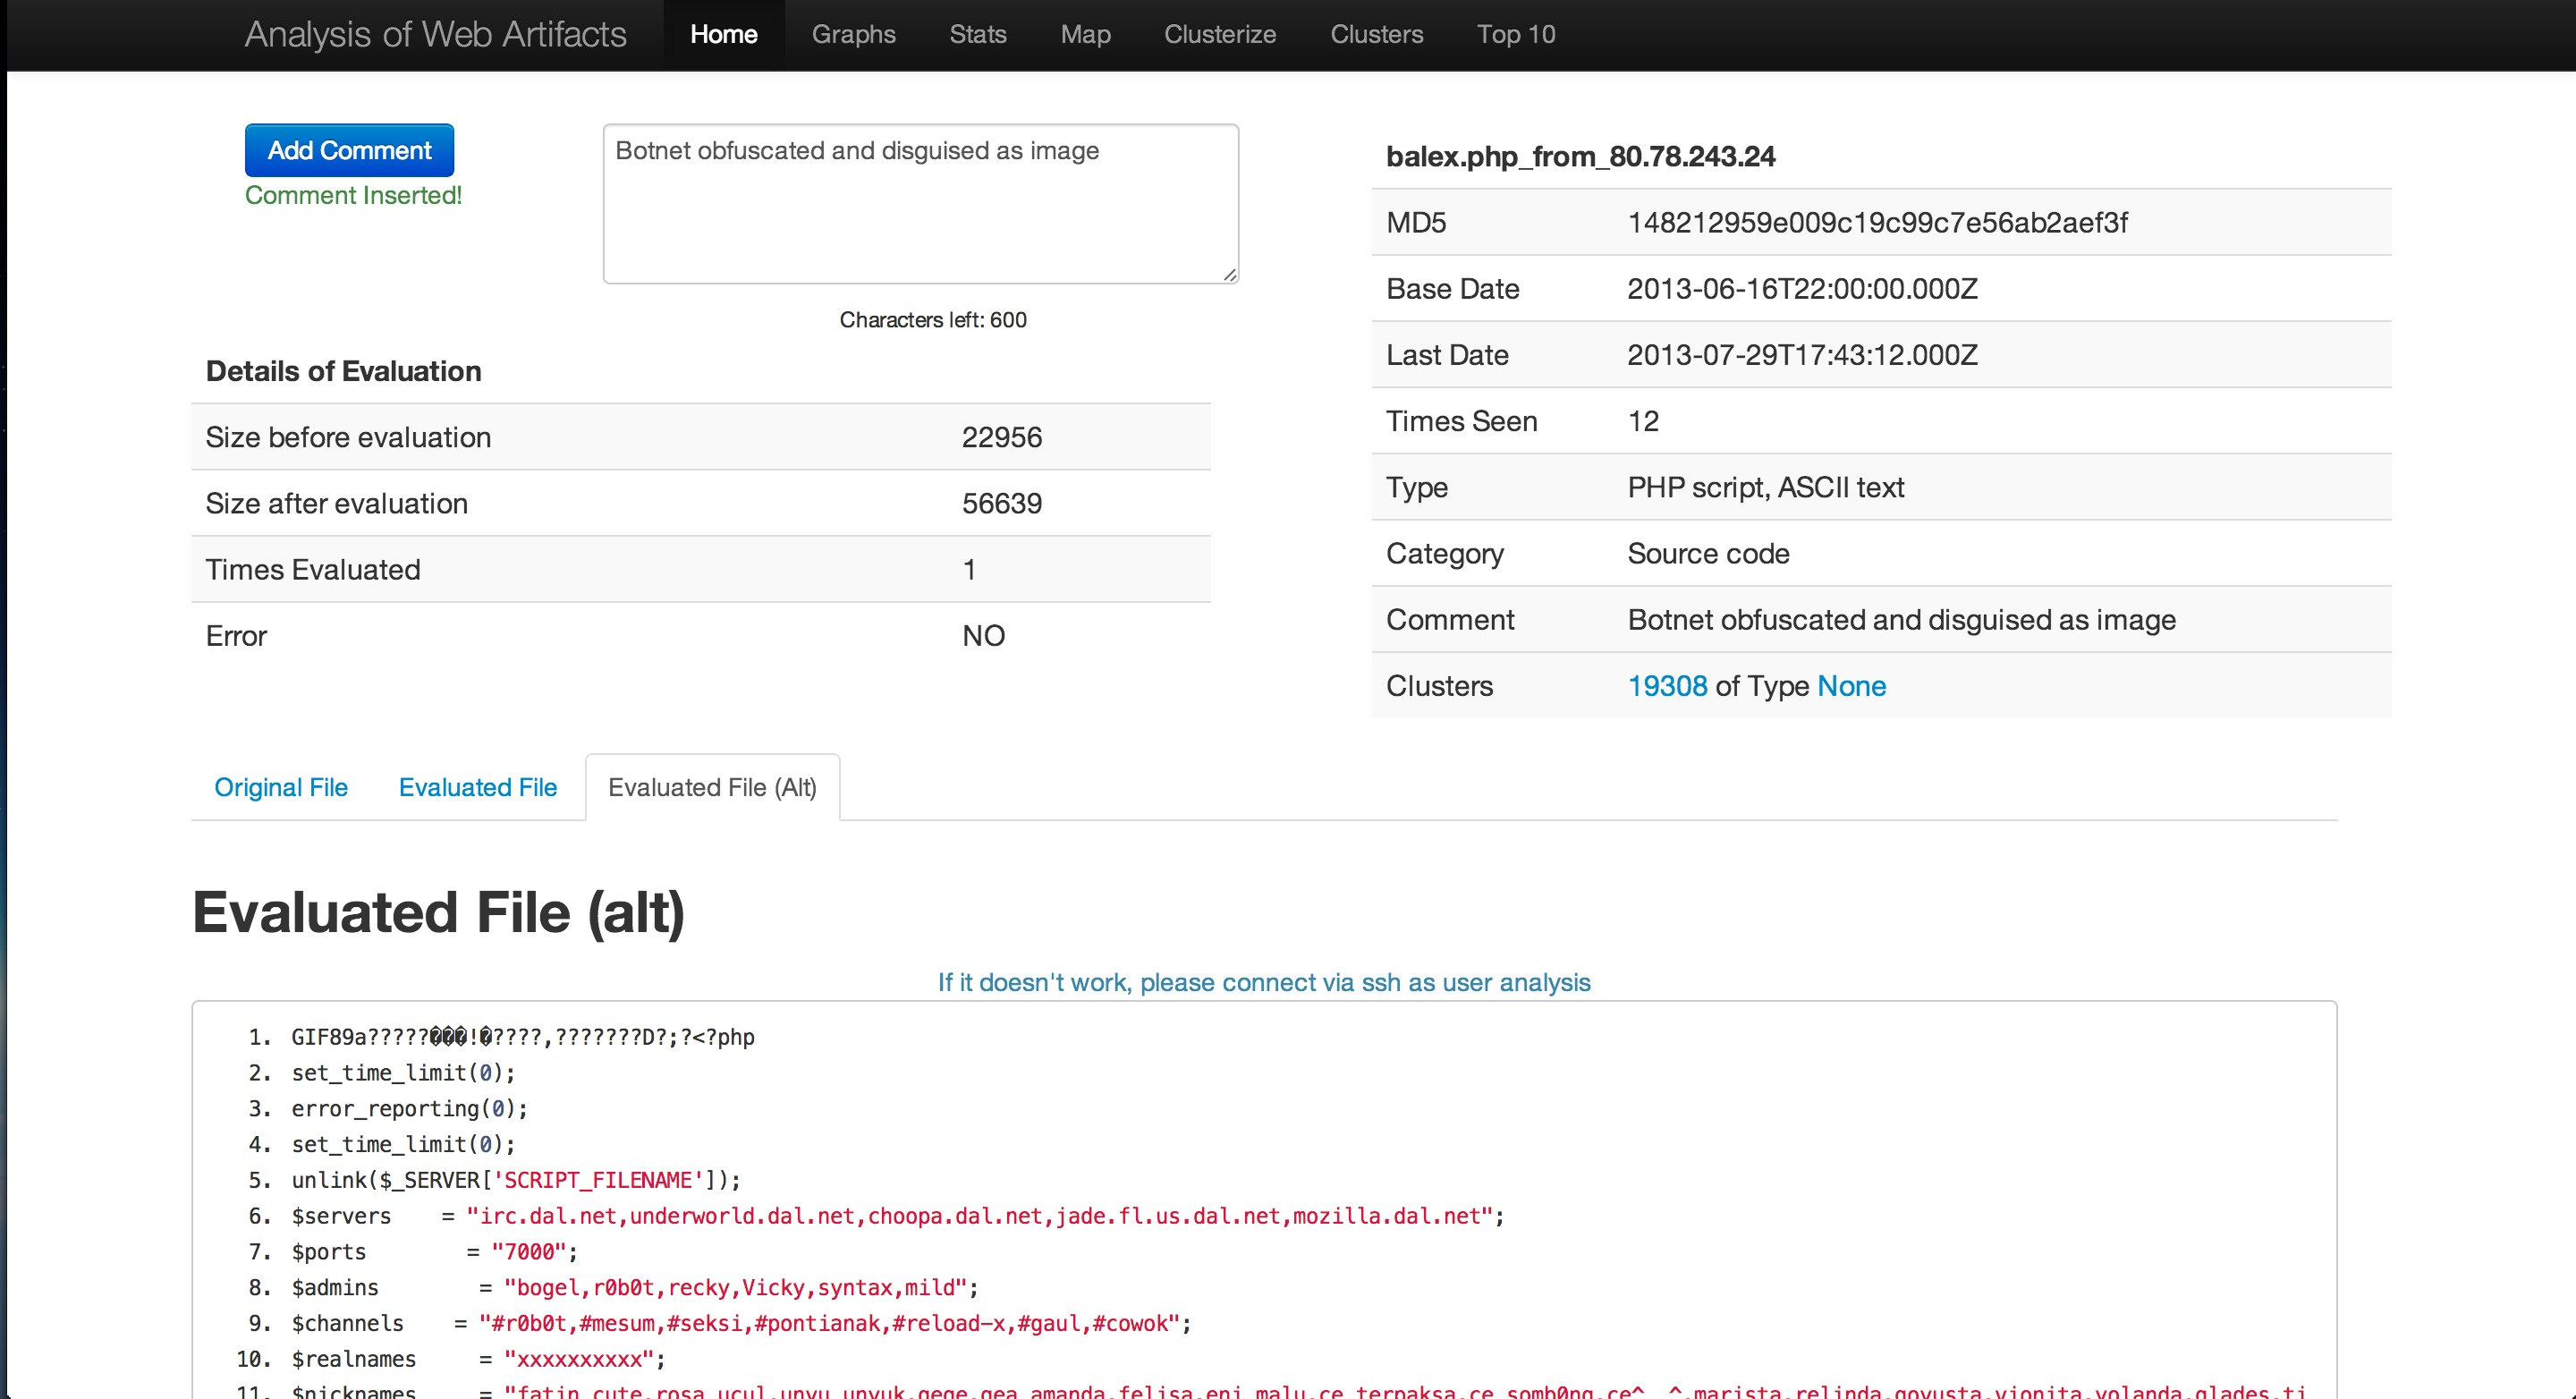
\includegraphics[width=1.0\linewidth]{Images/deobf_file.jpg}
  \caption{After deobfuscation}
  \label{fig:sub2}
\end{subfigure}
\caption{Example of the Single File web page}
\label{fig:deobfDouble}
\end{figure}



